\section{Discretization of the Electrophysiology Models}\label{sec:discretization}

The partial and ordinary differential equations described in the last section contain spatial and temporal derivatives that have to be discretized to be solved numerically. For temporal derivatives, we use timestepping schemes, for spatial derivatives, we employ the finite element method.

In this section, we describe the discretization of the subcellular and electrophysiology models that were presented in the last section. A description of the discretization of the solid mechanics model follows in \cref{sec:discretization_mechanics}.

We begin with the discretization in time in \cref{sec:discretization_monodomain}, followed by the spatial discretization for the monodomain (\cref{sec:discretization_diffusion,sec:mass_lumping}) and multidomain models (\cref{sec:discretization_multidomain,sec:discretization_body_domain}).

\subsection{Discretization of the Monodomain Model}\label{sec:discretization_monodomain}

Electrophysiology models typically consists of a reaction-diffusion equation. The diffusion term describes the electric conduction in the tissue and the reaction term includes the subcellular model. In our model, the monodomain equation  \cref{eq:monodomain} used in the fiber based description and the second multidomain equation \cref{eq:multidomain2} are equations of this type.

This type of partial differential equation is often solved using operator splitting schemes. A first order operator splitting scheme is Godunov splitting \cite{Godunov2003}. It was used for the solution of the chemo-electro-mechanical model in \cite{Roehrle2012}. In addition to Godunov splitting, we also employ the second order accurate Strang splitting scheme \cite{Strang1968}.

In the following, the application of these two schemes is illustrated for the monodomain equation \cref{eq:monodomain}. The right hand sides of the diffusion and reaction terms are denoted in short as $\mathcal{L}_1$ and $\mathcal{L}_2$:%
\begin{align*}
  \mathcal{L}_1(V_m) := \dfrac{1}{A_m\,C_m} \sigma_\text{eff}\dfrac{\partial^2 V_m}{\partial x^2}, &&
  \mathcal{L}_2(V_m) := -\dfrac{1}{C_m} I_\text{ion}(V_m,\bfy).
\end{align*}
%
Then, the monodomain equation takes the form:
%
\begin{align}\label{eq:monodomain_operator_splitting}
  \p{V_m}{t} = \mathcal{L}_1(V_m) + \mathcal{L}_2(V_m).
\end{align}

A timestepping scheme is constructed that starts with a given initial value $V_m^{(0)}$ and computes solution values $V_m^{(i)}$ at discrete points in time $t^{(i)} = i\cdot\dt$ with a fixed timestep width $\dt$.
Godunov splitting proceeds by alternatingly performing steps in the two directions of the right hand sides $\mathcal{L}_1$ and $\mathcal{L}_2$. In the first substep per iteration, an intermediate value $V_m^{\ast}$ is calculated, which is used as starting point for the second substep. Each of the substeps are performed using independent timestepping scheme, e.g., the explicit Euler scheme:
%
\begin{subequations}\label{eq:monodomain_godunov}
  \begin{align}
    V_m^{\ast} &= V_m^{(i)} + \dt \mathcal{L}_1(V_m^{(i)},t^{(i)}),\\[4mm]
    V_m^{(i+1)} &= V_m^{\ast} + \dt \mathcal{L}_2(V_m^{\ast},t^{(i)})
  \end{align}
\end{subequations}

Strang splitting uses a similar approach with three substeps per timestep and two intermediate values $V_m^{\ast}$ and $V_m^{\ast\ast}$:
%
\begin{subequations}\label{eq:monodomain_strang}
  \begin{align}
    V_m^{\ast} &= V_m^{(i)} + \dfrac{\dt}{2} \mathcal{L}_1(V_m^{(i)},t^{(i)}),\\[4mm]
    V_m^{\ast\ast} &= V_m^{\ast} + \dt \mathcal{L}_2(V_m^{\ast},t^{(i)}),\\[4mm]
    V_m^{(i+1)} &= V_m^{\ast\ast} + \dfrac{\dt}{2} \mathcal{L}_1(V_m^{\ast\ast},t_{(i)}+\dfrac12 \dt).
  \end{align}
\end{subequations}
%
% stuff needed to create the plot
%\definecolor{vred}{RGB}{170,0,0}
%\definecolor{vyellow}{RGB}{212,170,0}
%\definecolor{vgreen}{RGB}{0,170,0}
%\begin{equation*}
%  \begin{array}{lll}
%    \frac{\partial}{\partial t} V_m  = \textcolor{vred}{c_1 \frac{\partial^2}{\partial x^2} V_m }\\[4mm]
%    \frac{\partial}{\partial t} \bfy = \textcolor{vyellow}{G(V_m,\bfy)}\\[4mm]
%    \frac{\partial}{\partial t} V_m = \textcolor{vyellow}{c_2\,I_\text{ion}(V_m,\bfy)}\\[4mm]
%    \textcolor{vyellow}{\dt_\text{0D}}\quad
%    \textcolor{vred}{\dt_\text{1D}}\quad
%    \dt_\text{splitting}\quad
%    \textcolor{vgreen}{\dt_\text{3D}}\quad
%    t^{(i)}, t^{(i)} + \dt_\text{splitting}/2, t^{(i)} + \dt_\text{splitting} ...\\[4mm]
%    t^{(i)} + \textcolor{vgreen}{\dt_\text{3D}}\\[4mm]
%    t^{(i+1)}
%  \end{array}
%\end{equation*}
%\textcolor{vyellow}{0D:}
%\textcolor{vred}{1D:}
%\textcolor{vgreen}{3D:}

Note that each substep can either be executed as a single timestep of the chosen method as in \cref{eq:monodomain_godunov,eq:monodomain_strang} or divided into several steps with timestep widths $\dt_{0D}$ (for the 0D subcellular model represented by $\mathcal{L}_1$) and $\dt_{1D}$ (for the diffusion equation represented by $\mathcal{L}_2$).

\Cref{fig:splitting_schemes} visualizes both splitting schemes applied to the monodomain equation. 
The yellow arrows correspond to the solution of the 0D subcellular model. The red arrows correspond to the solution of the 1D diffusion equation. The timestep width of one splitting step is $\dt_\text{splitting}$. Depending on how the timestep widths are chosen in relation to each other, different numbers of subcycles are used in the solution of the 0D and 1D problems.

\begin{figure}%
  \centering%
  \begin{subfigure}[t]{0.48\textwidth}%
    \centering%
    \def\svgwidth{\textwidth}
    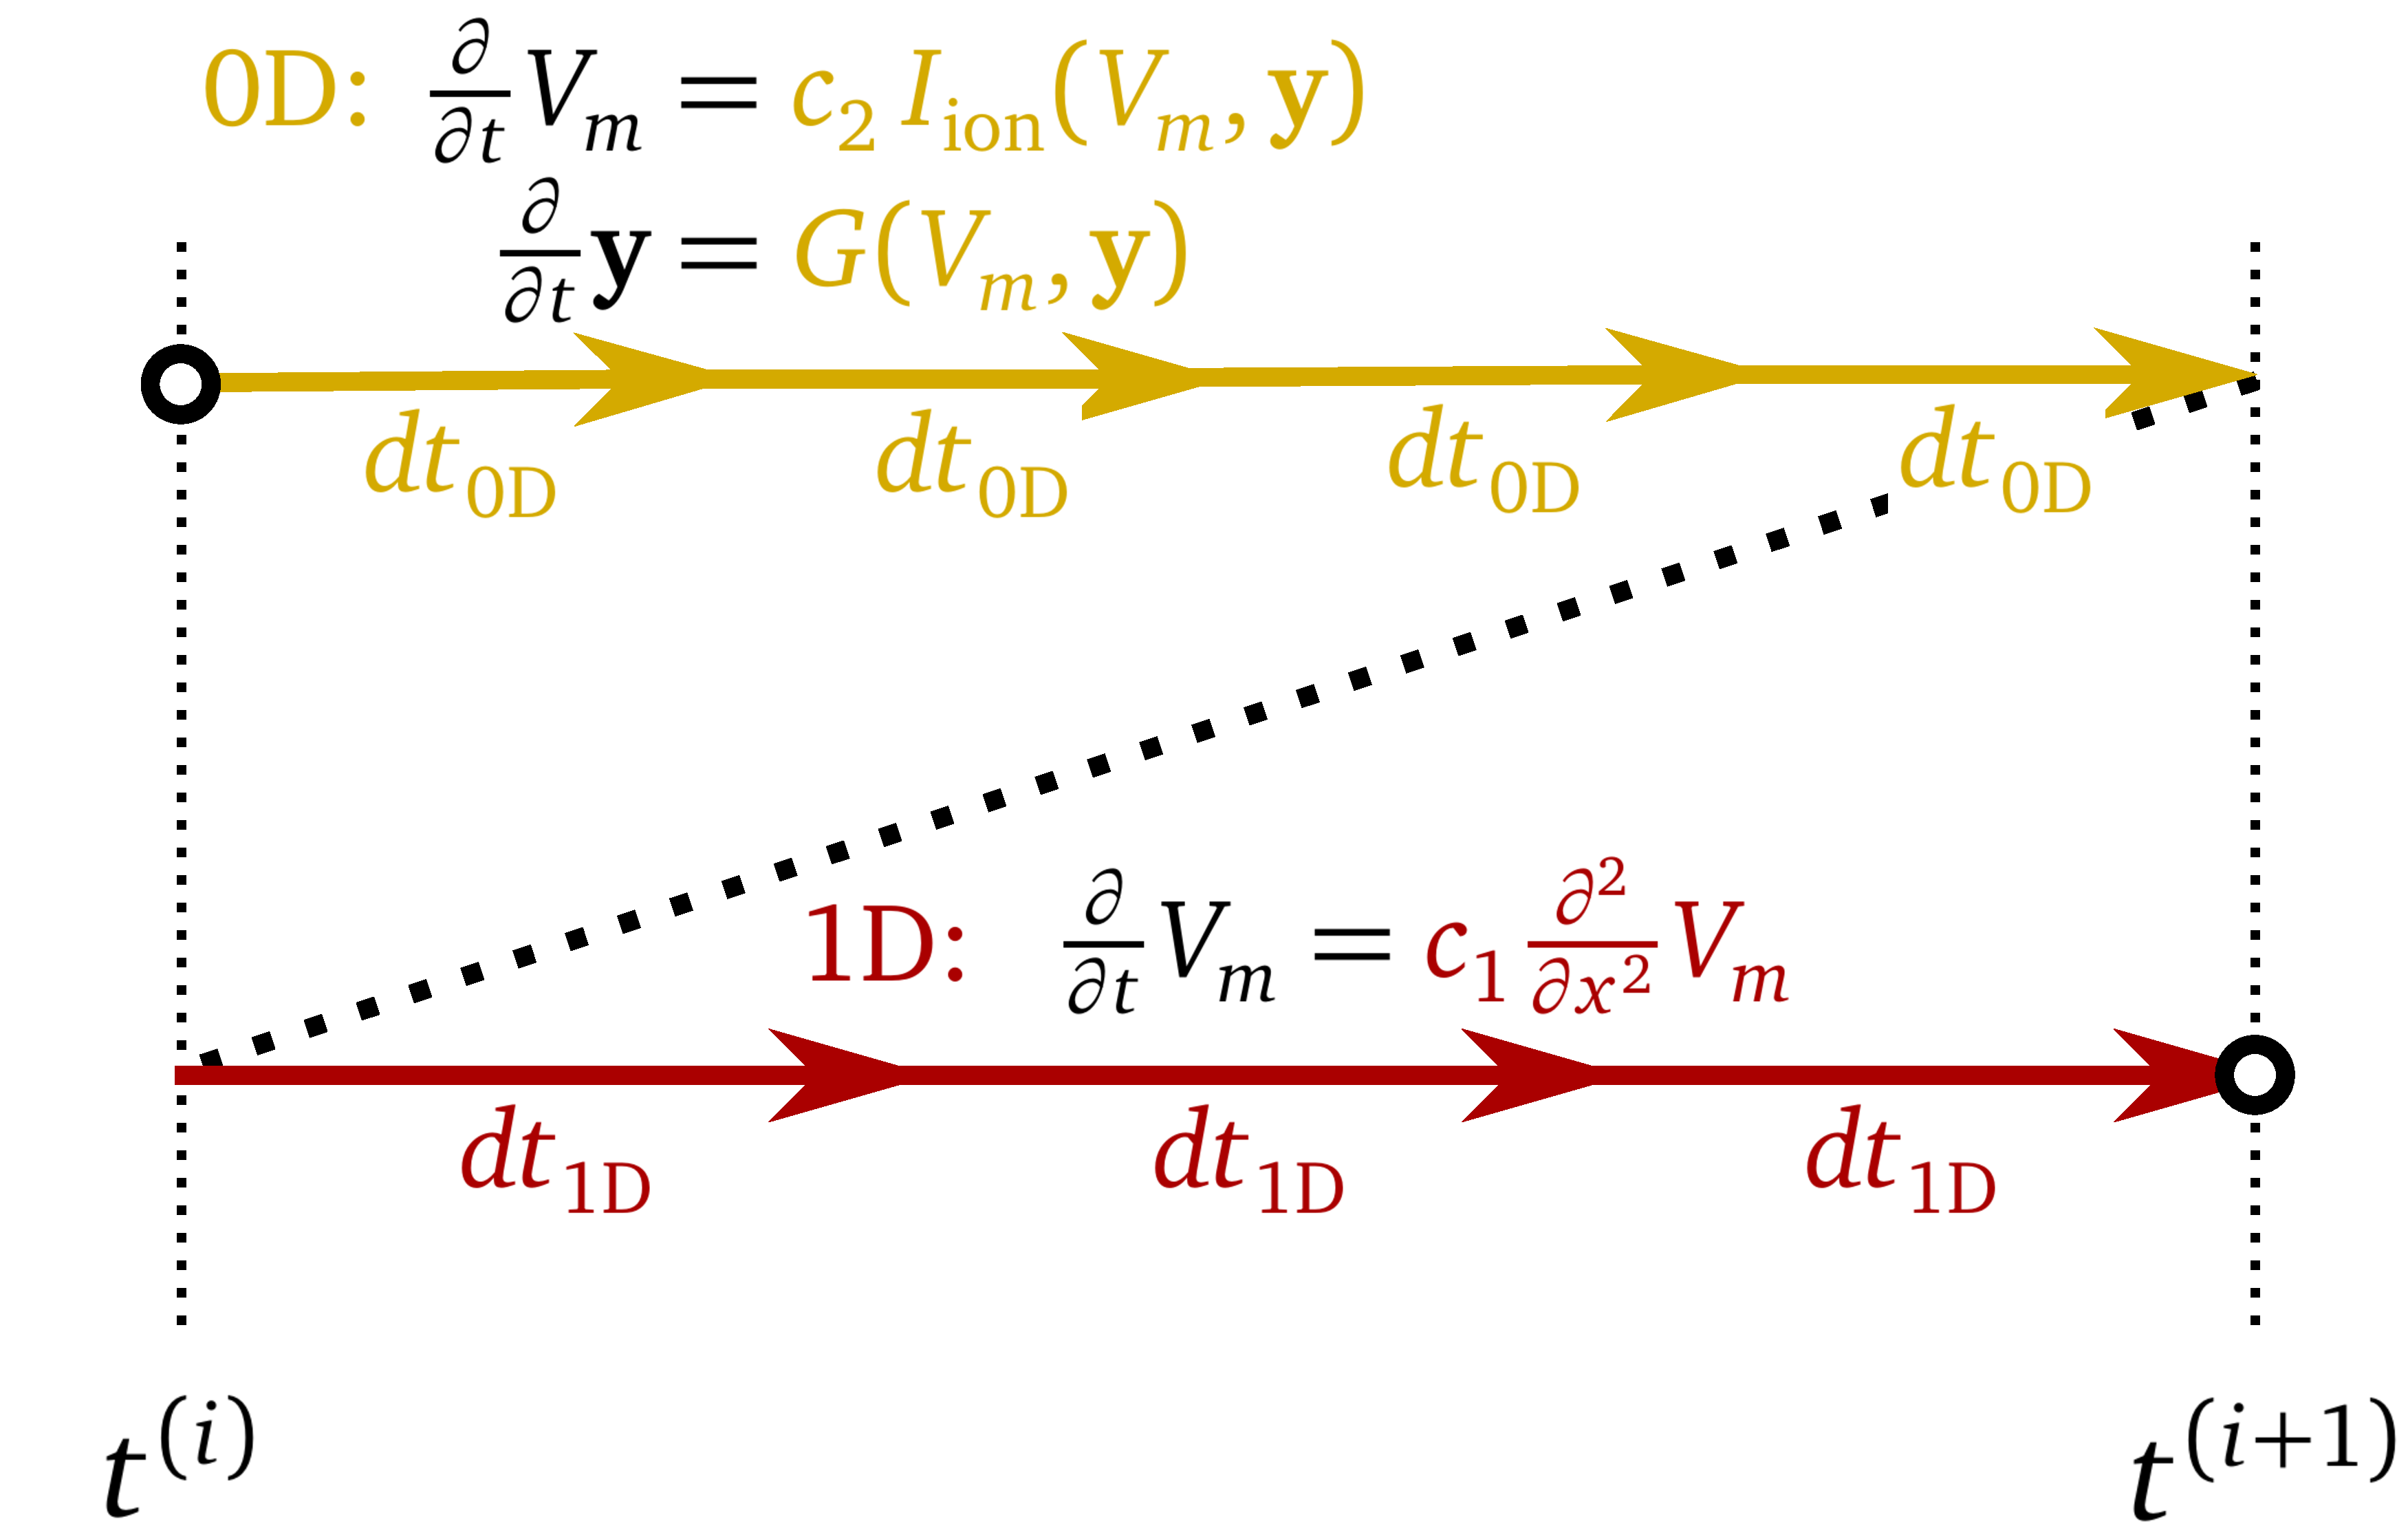
\includegraphics[width=\textwidth]{images/theory/godunov_splitting.pdf}
    \caption{The Godunov splitting uses two substeps: 0D, 1D.}%
    \label{fig:godunov_splitting}%
  \end{subfigure}
  \quad
  \begin{subfigure}[t]{0.48\textwidth}%
    \centering%
    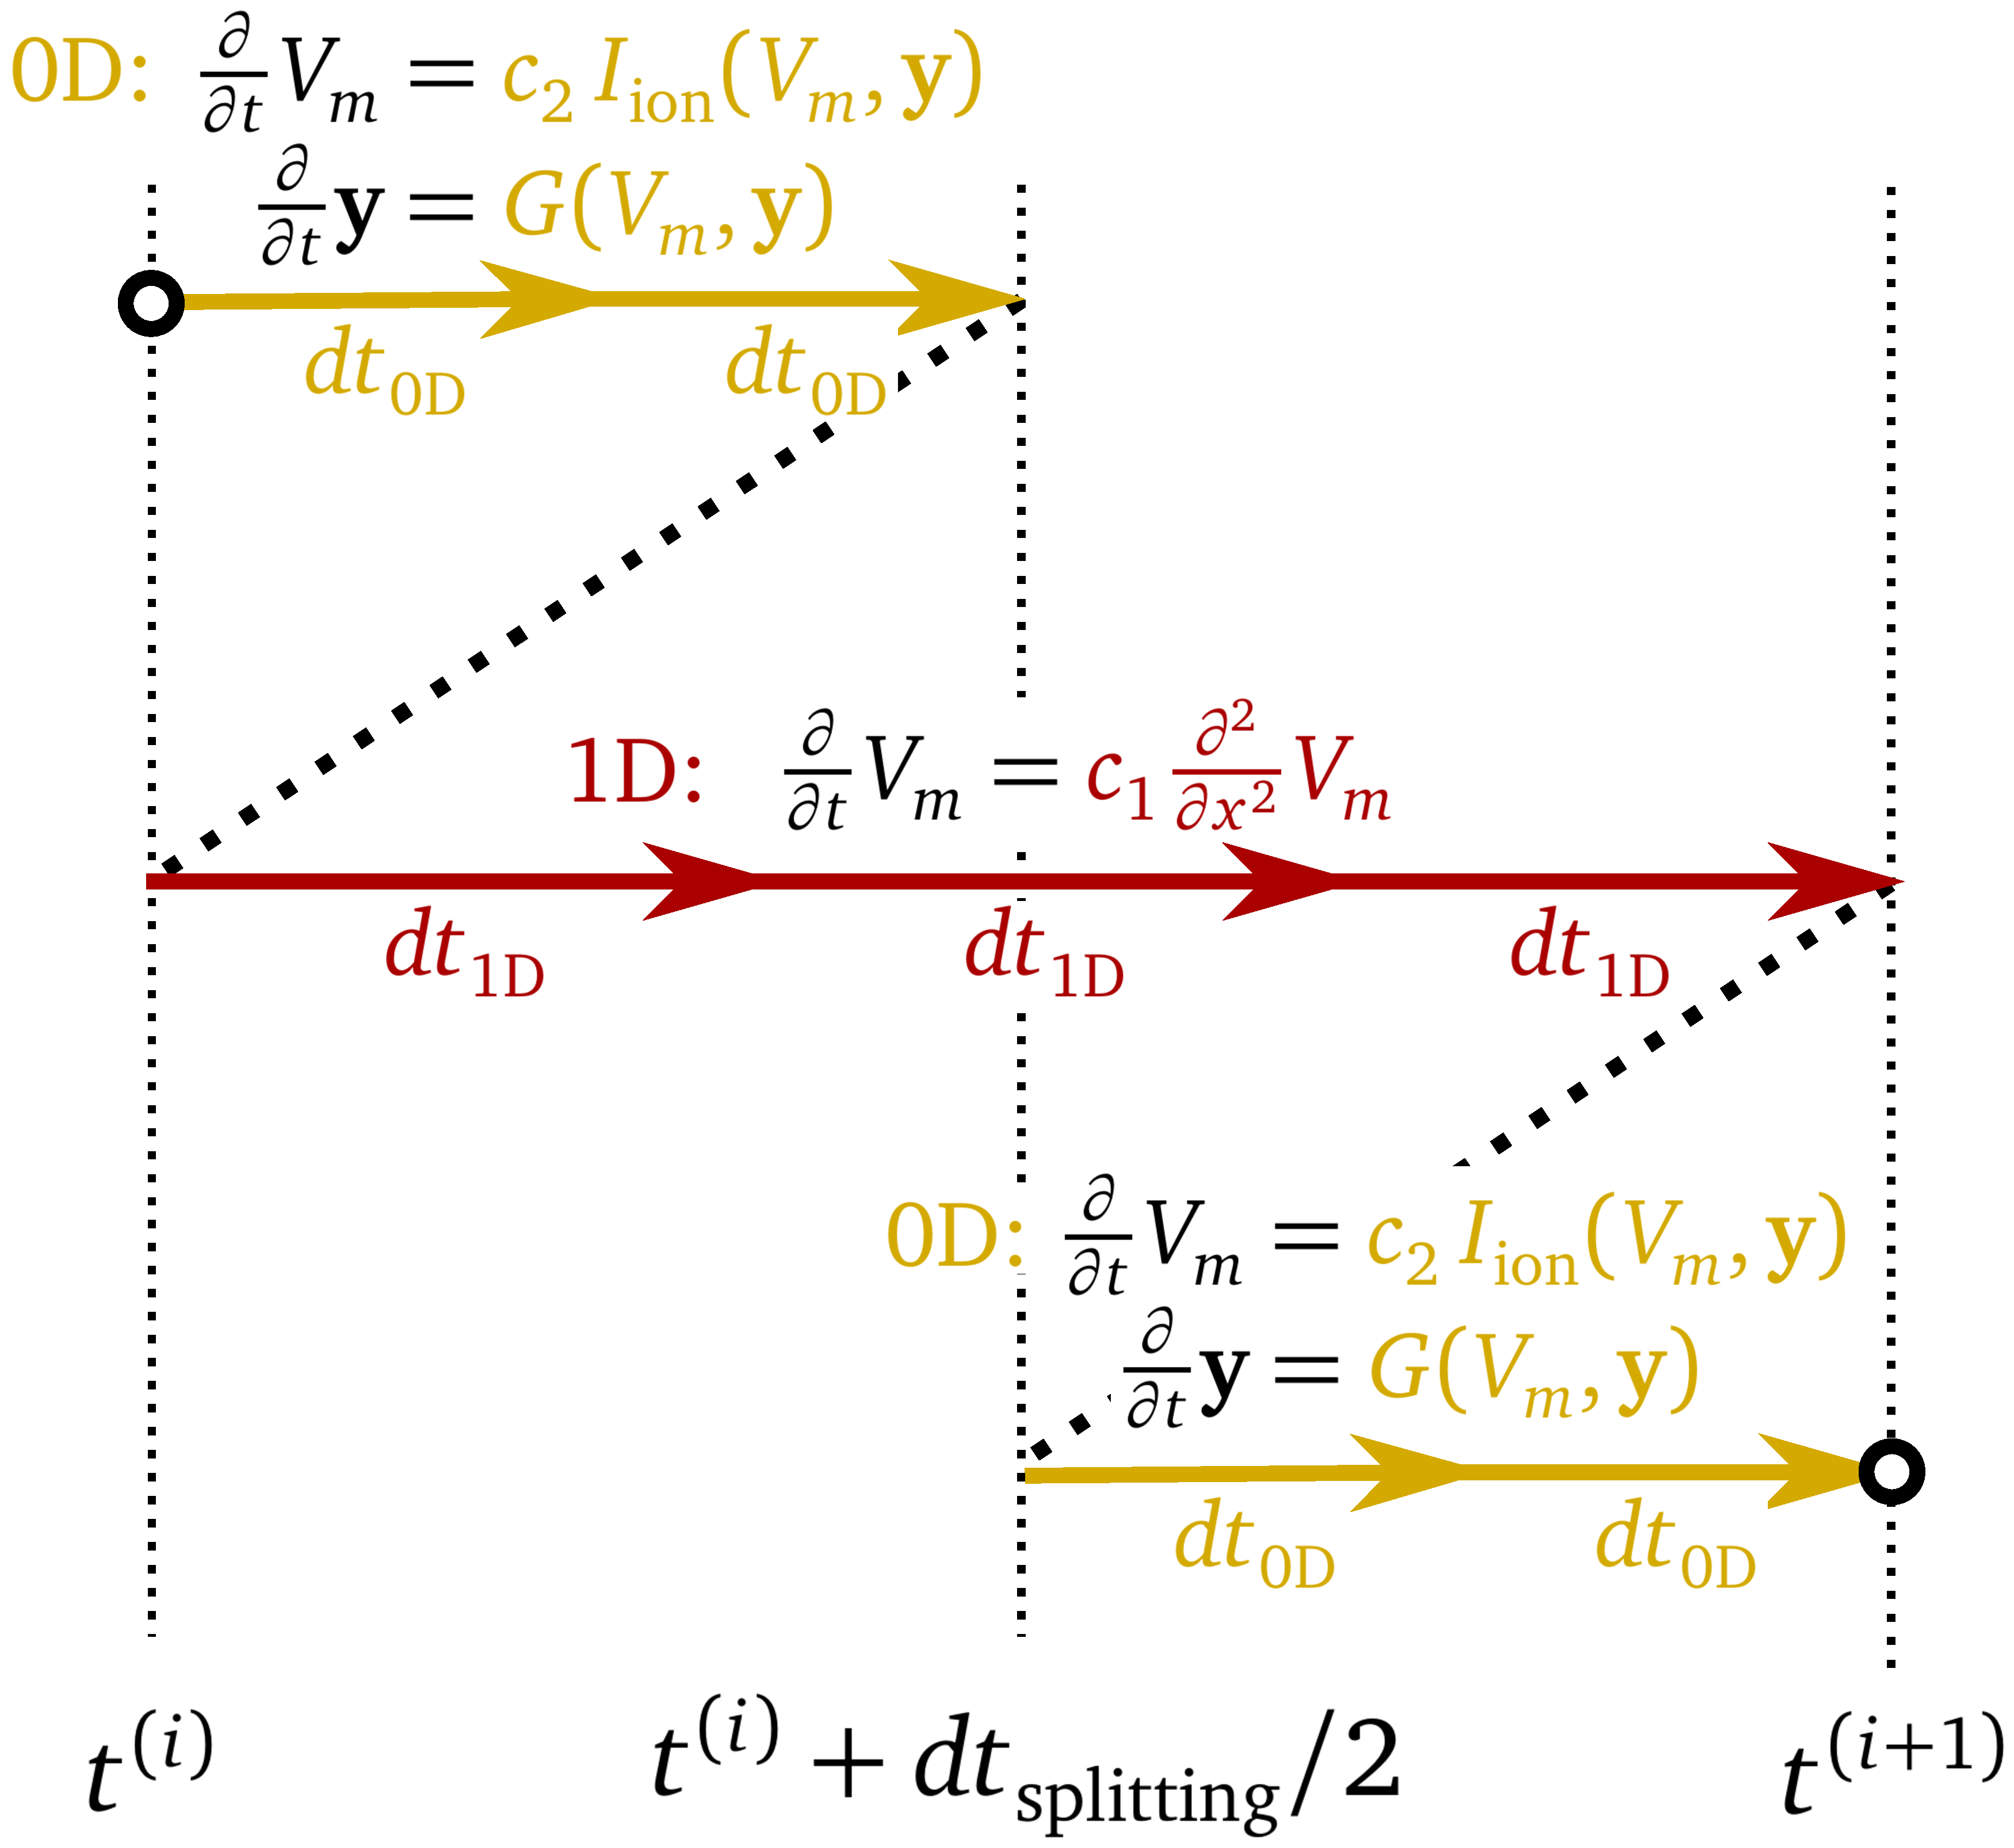
\includegraphics[width=\textwidth]{images/theory/strang_splitting.pdf}
    \caption{The Strang splitting uses three substeps: 0D, 1D, 0D.}%
    \label{fig:strang_splitting}%
  \end{subfigure}
  \caption{Godunov and Strang splitting schemes that are used to solve the monodomain equation. The equation is split into a reaction part (0D,yellow) and a diffusion part (1D,red) and these parts are solved alternatingly. The visualizations show one splitting timestep starting at the left circle and completing at the right circle.}%
  \label{fig:splitting_schemes}%
\end{figure}%

Instead of the explicit Euler method in \cref{eq:monodomain_godunov,eq:monodomain_strang}, other timestepping methods can be used for the substeps. 
We use the following schemes, which are listed as single steps for the generic ODE ${\p V_m / \p t = \mathcal{L}(V_m,t)}$:
\begin{subequations}\label{eq:ode_solver_schemes}
  \begin{align}
    V_m^{(i+1)} &= V_m^{(i)} + \dt \mathcal{L}(V_m^{(i)},t^{(i)}), \label{eq:explicit_euler}\\[4mm]
    V_m^{(i+1)} &= V_m^{(i)} + \dfrac{\dt}{2}\Big(
      \mathcal{L}(V_m^{(i)},t^{(i)}) + \mathcal{L}\big(V_m^{(i)} + \dt \mathcal{L}(V_m^{(i)},t^{(i)}),t^{(i+1)}\big)\Big), \label{eq:heun}\\[4mm]
    V_m^{(i+1)} &= V_m^{(i)} + \dt \mathcal{L}(V_m^{(i+1)},t^{(i+1)}), \label{eq:implicit_euler}\\[4mm]
    V_m^{(i+1)} &= V_m^{(i)} + \dfrac{\dt}{2}\Big(
      \theta\,\mathcal{L}(V_m^{(i+1)},t^{(i+1)}) + (1-\theta)\,\mathcal{L}(V_m^{(i)},t^{(i)})\Big).\label{eq:crank_nicolson}
  \end{align}
\end{subequations}
%
Here, \cref{eq:explicit_euler} is the first-order accurate explicit Euler scheme, \cref{eq:heun} is the second-order accurate Heun scheme, \cref{eq:implicit_euler} is the first order accurate implicit Euler scheme, and \cref{eq:crank_nicolson} is the Crank-Nicolson scheme \cite{CrankNicolson1947}, which for $\theta=0$ equals the explicit Euler and for $\theta=1$ equals the implicit Euler scheme. For $\theta=\frac12$, it is second order accurate. An advantage of the implicit schemes in \cref{eq:implicit_euler,eq:crank_nicolson} is, that, for our considered diffusion problems, they are unconditionally stable. A disadvantage is, that a linear equation has to be solved in every timestep.

A second order accurate timestepping scheme yields a faster decrease of the numerical error with decreasing step size and, thus, in many cases allows a larger step size than a first order scheme.
To obtain a second order scheme for the monodomain equation, we use Strang splitting (\cref{eq:monodomain_strang}) with the Crank-Nicolson scheme (\cref{eq:crank_nicolson}) for the diffusion term $\mathcal{L}_1$ and Heun's method (\cref{eq:heun}) for the reaction term $\mathcal{L}_2$. In the subcellular model, the system of ODEs with state vector $\bfy$ given in \cref{eq:subcellular} is solved with Heun's method along with the equation in terms of $V_m$.

Next, the spatial derivatives in the diffusion part $\mathcal{L}_2$ of the split equation have to be discretized. Then, both the multidomain and the fiber based models can be solved using the splitting scheme.

\subsection{Discretization of the Diffusion and Laplace Equations}\label{sec:discretization_diffusion}

For the spatial discretization, we first derive the finite element formulation for a generic parabolic diffusion equation in a domain $\Omega\subset\R^d$ of arbitrary dimensionality $d$. Then, specialization to 1D yields the formulation for the monodomain equation. Considering a 3D domain, the formulation is an important building block for the discretization of the multidomain model. This is shown in more detail in a later section, \cref{sec:discretization_multidomain}

We consider the following diffusion problem in the variable $u: \Omega \times [0,t_\text{end}] \to \R$ with Neumann boundary conditions on a part of the boundary $\Gamma_f \subset ∂\Omega$ with normal vector $\bfn$:
\begin{align*}
  \p{u}{t} &= \div(\bfsigma \grad u), &(\bfsigma\,\grad u) \cdot \bfn &= f \quad \text{on }\Gamma_f, & (\bfsigma\,\grad u) \cdot \bfn &= 0 \quad \text{on } ∂Ω\backslash \Gamma_f.
\end{align*}
We discretize the temporal derivative using the Crank-Nicolson scheme as in \cref{eq:crank_nicolson}. Following the procedure of the Galerkin finite element formulation with the Hilbert space $H^1_0(\Omega)$ of test functions $\phi$ that are zero on the boundary, we arrive at the following weak form:
%
\begin{align*}
  \ds\int_Ω \big(\theta\,∇\cdot(\bfsigma ∇ \bfu^{(i+1)})  + (1-\theta)\,∇\cdot(\bfsigma ∇ u^{(i)})\big)\,\phi \,\d\bfx &&\\
    \qquad = \dfrac{1}{\dt} \ds\int_Ω(u^{(i+1)} - u^{(i)})\,\phi\,\d\bfx, &&\qquad \forall \phi \in H^1_0(\Omega).
\end{align*}
For brevity, we express divergence and gradient using the nabla operator. 

To discretize the weak form in space, we choose a function space $V_h = \text{span}\{\varphi_j \mid j = 1, \dots, N\}$ to represent the solution as $u = \sum_{j=1}^N u_j \phi_j$. Applying the divergence theorem, we obtain:
\begin{equation}\label{eq:diffusion_helper1}
  \begin{array}{l}
    \ds\sum\limits_{j=1}^{N} \big(\theta\,u_j^{(i+1)} + (1-\theta)\,u_j^{(i)}\big)  
    \left(-\ds\int_Ω \bfsigma\,∇\varphi_j\cdot ∇\varphi_k \,\d\bfx + \ds\int_{∂Ω} \big(\bfsigma\,∇\varphi_j\cdot \bfn\big)\,\varphi_k \,\d\bfx  \right) \\
      \quad = \dfrac{1}{\dt} \sum\limits_{j=1}^{N} \big(u_j^{(i+1)} - u_j^{(i)}\big) \ds\int_Ω \varphi_j\,\varphi_k\,\d\bfx, \qquad \forall k = 1,\dots, N.
  \end{array}
\end{equation}
This iteration step can be written in matrix notation in terms of the vectors of unknowns $\bfu^{(i)}=(u^{(i)}_0,\dots,u^{(i)}_N)^\top$ at timestep $i$:%
\begin{align*}
  \bfA\,\bfu^{(i+1)} = \bfb(\bfu^{(i)}).
\end{align*}
The system matrix $\bfA$ and the right hand side $\bfb$ are given by:
\begin{align*}
  \bfA &= \theta\,(\bfK_{\bfsigma} + \bfB_{\bfsigma}) -\dfrac{1}{\dt}\bfM, &
  \bfb &= \big((\theta-1)\,(\bfK_{\bfsigma} + \bfB_{\bfsigma}) - \dfrac{1}{\dt} \bfM \big)\,\bfu^{(i)}.
\end{align*}
The formulation uses the standard stiffness matrix $\bfK_{\bfsigma}$, the matrix $\bfB_{\bfsigma}$ of the boundary integral and the mass matrix $\bfM$, whose components are defined as%
\begin{align}\label{eq:diffusion_matrices}
  \bfK_{\bfsigma,kj} &= -\ds\int_Ω (\bfsigma\, ∇\varphi_j)\cdot ∇\varphi_k \,\d\bfx,&
     \bfB_{\bfsigma,kj} &= \ds\int_{\Gamma_f} \big((\bfsigma\,∇\varphi_j)\cdot \bfn\big)\,\varphi_k \,\d\bfx,&
     \bfM_{kj} &= \ds\int_Ω \varphi_j\,\varphi_k\,\d\bfx.
\end{align}
Note that, after applying the divergence theorem, the definition of the stiffness matrix has a minus sign.

Next, we take into account the Neumann boundary condition $\bfsigma∇u\cdot \bfn = f$ on the boundary $\Gamma_f$. The flux $f$ over the boundary is discretized by $M$ separate ansatz functions $\psi_j$ on $\Gamma_f$ as $f = \sum_{j=1}^M f_j\, \psi_j$.
The flux values are summarized in a vector $\bff=(f_1,\dots,f_M)^\top$.
Plugging this into \cref{eq:diffusion_helper1} yields the following equation in matrix notation:%
\begin{align}\label{eq:diffusion_helper2}
  \tilde{\bfA}\,\bfu^{(i+1)} = \tilde{\bfb}(\bfu^{(i)}),  
\end{align}
with the system matrix $\tilde{\bfA}$ and right hand side $\tilde{\bfb}$: 
\begin{align*}
  \tilde{\bfA} &= \theta\,\bfK_{\bfsigma} -\dfrac{1}{\dt}\bfM, &
    \tilde{\bfb} &= \big((\theta-1)\,\bfK_{\bfsigma} - \dfrac{1}{\dt} \bfM \big)\,\bfu^{(i)} - \bfB_{\Gamma_f}\,\big(\theta\,\bff^{(i+1)} + (1-\theta)\,\bff^{(i)}\big),
\end{align*}
and the boundary matrix $\bfB_{\Gamma_f}$ given by:
\begin{align}\label{eq:definition_boundary_matrix}
  \bfB_{\Gamma_f,kj} &= \ds\int_{\Gamma_f} \psi_j\,\varphi_k \,\d\bfx.
\end{align}
Note that incorporating the Neumann boundary conditions in the weak form corresponds to the following exchange of the boundary matrices $\bfB_\sigma$ and $\bfB_{\Gamma_f}$:%
\begin{align}\label{eq:boundary_relation}
  \bfB_\sigma\,\bfu = \bfB_{\Gamma_f}\,\bff.
\end{align}
%


\Cref{eq:diffusion_helper2} is used to solve the diffusion part of the monodomain equation given in \cref{eq:monodomain} after inserting the corresponding constant prefactors.

When deriving or implementing new models or optimizing solver code, it is often beneficial to study certain effects in isolation. It can help to use a toy problem such as the simple Laplace problem $Δu = 0$, possibly with Neumann boundary condition $\partial u/\partial \bfn = f$. 
By specializing the formulation in \cref{eq:diffusion_helper2} accordingly, we obtain the system
%
\begin{align*}
  (\bfK_\bfI + \bfB_\bfI)\,\bfu = \bfzero
\end{align*}
for the case without boundary condition (set $\bfB_\bfI$ to zero to assume homogenous Neumann boundaries) or
\begin{align}\label{eq:discretization_laplace}
  \bfK_\bfI\,\bfu = -\bfB_{\Gamma_f}\,\bff
\end{align}
to include the formulated Neumann boundary condition.

\subsection{Using Mass Lumping for Implicit Timestepping}\label{sec:mass_lumping}
Implicit timestepping schemes such as implicit Euler or the Crank-Nicoloson scheme for $\theta=\frac12$ need to solve a linear equation in every timestep.
Assuming homogeneous Neumann boundary conditions for simplicity, the iteration step of the canonical Crank-Nicolson scheme follows from \cref{eq:diffusion_helper2}:
\begin{subequations}\label{eq:lumping_crank_nicolson}
  \begin{align}
    \big(\dfrac1{2}\bfK-\dfrac{1}{\dt}\bfM\big)\, \bfu^{(i+1)} &= \big(-\dfrac12{\bfK} - \dfrac{1}{\dt}\bfM\big)\, \bfu^{(i)}\label{eq:lumping_crank_nicolson_1}\\[4mm]
    \Leftrightarrow \quad (\bfI - \dfrac{\dt}{2}\,\bfM^{-1}\bfK)\,\bfu^{(i+1)}&= (\bfI + \dfrac{\dt}{2}\,\bfM^{-1}\bfK)\,\bfu^{(i)}.\label{eq:lumping_crank_nicolson_2}
  \end{align}
\end{subequations}
For the implicit Euler method, we obtain:%
\begin{subequations}\label{eq:lumping_implicit_euler}
  \begin{align}
    \ds(\bfK-\frac{\bfM}{\dt})\,\bfu^{(i+1)} &=\,\ds -\frac{\bfM}{\dt}\bfu^{(i)}\label{eq:lumping_implicit_euler_1}\\[4mm]
    \Leftrightarrow \quad (\bfI - \dt\,\bfM^{-1}\bfK)\,\bfu^{(i+1)}&= \,\bfu^{(i)}.\label{eq:lumping_implicit_euler_2}
  \end{align}
\end{subequations}
Both iteration steps in \cref{eq:lumping_crank_nicolson_1,eq:lumping_crank_nicolson_2} and in \cref{eq:lumping_implicit_euler_1,eq:lumping_implicit_euler} are equivalent, as the second equation follows from the first one by left multiplication of $(-\dt \bfM^{-1})$. In the second equations, the matrices to be multiplied are created by a sum of the unity matrix $\bfI$ and another matrix term that is scaled by the potentially small timestep width $\dt$. For the implicit Euler in \cref{eq:lumping_implicit_euler_2}, the matrix on the right hand side even reduces to the identity matrix. This is preferred over the first iteration steps in \cref{eq:lumping_crank_nicolson_1,eq:lumping_implicit_euler_1} as it leads to better conditioned matrix-vector multiplications.

The required inversions of the mass matrix cannot be carried out explicitly as the inversion would fill in numerous matrix entries and eliminate the sparse structure. This is not feasible for highly resolved meshes with a large number of degrees of freedom. Instead, \emph{mass lumping} is used, where the mass matrix $\bfM$ is approximated by a diagonal matrix with diagonal entries equal to the row sums in $\bfM$ \cite{Hinton1976}. Thus, multiplication with the inverse mass matrix corresponds to a rescaling of columns by the inverse lumped diagonal entries.

\subsection{Discretization of the Multidomain Model}\label{sec:discretization_multidomain}
With the prerequisites of temporal discretization in \cref{sec:discretization_monodomain} and the finite element formulation of a diffusion equation in \cref{sec:discretization_diffusion}, we can now discretize the multidomain model. Since this has not been previously done in literature using the finite element method, the subsequent derivation is more detailed.

The first multidomain equation given in \cref{eq:multidomain1} yields the following form after applying the finite element derivation in \cref{eq:diffusion_helper2}:
%
\begin{align}\label{eq:multidomain_discretization_helper_multidomain1}
  \big(\bfK_{\bfsigma_e + \bfsigma_i} + \bfB_{\bfsigma_e + \bfsigma_i}\big)\,\bfphi_{e} +  \s{k=1}{N_\text{MU}} f_r^k \big(\bfK_{\bfsigma_i^k} + \bfB_{\bfsigma_i^k}\big)\,\bfV_m^k = 0.  
\end{align}
Here, $\bfphi_{e}$ and $\bfV_m^k$ are the vectors of degrees of freedom for the extracellular potential $\phi_e$ and membrane voltage $V_m^k$ of compartment $k$. The matrices are defined by \cref{eq:diffusion_matrices} and do not yet include the boundary conditions.
The subscripts of the stiffness matrices $\bfK$ and boundary integral matrices $\bfB$ refer to the anisotropy tensors that occur in their definitions.

The diffusion part of the second multidomain equation, \cref{eq:multidomain2}, discretized with Crank-Nicolson, yields the system%
\begin{align}\label{eq:multidomain_discretization_helper_multidomain2}
  \bfA\,\mat{\bfV_m^{k,(i+1)}\\ \bfphi_{e}^{(i+1)}} = \bfb,  
\end{align}
%
with the $1 \times 2$ block system matrix $\bfA$ and right hand side vector $\bfb$ given by:%
\begin{subequations}\label{eq:multidomain_discretization_helper_multidomain3}
\begin{align}
   \bfA &= \matt{
      \dfrac{\theta}{A_m^k\,C_m^k}(\bfK_{\bfsigma_i^k} + \bfB_{\bfsigma_i^k}) -\dfrac{1}{\dt}\bfM & \quad
      \dfrac{\theta}{A_m^k\,C_m^k}(\bfK_{\bfsigma_i^k} + \bfB_{\bfsigma_i^k})
    }, \\[4mm]
    \bfb &= \Big( \dfrac{\theta-1}{A_m^k\,C_m^k}(\bfK_{\bfsigma_i^k} + \bfB_{\bfsigma_i^k}) - \dfrac{1}{\dt}\bfM\Big)\,\bfV_m^{k,(i)} 
      + \dfrac{\theta - 1}{A_m^k\,C_m^k}(\bfK_{\bfsigma_i^k} + \bfB_{\bfsigma_i^k})\,\bfphi_e^{(i)}.
\end{align}
\end{subequations}

A separate instance of this equation holds for every compartment $k$. Again, the integrals over the boundary are still present in the $\bfB_{\bfsigma_i^k}$ matrices.
To resolve this and to close the formulation, we have to consider the fluxes over the boundary of all involved unknowns and to replace them using the boundary conditions.

One required boundary conditions to solve the multidomain model without body domain is given in \cref{eq:multidomain_bc1}. The boundary condition for compartment $k$ in terms of the intracellular potential $\phi_i^k$,
%
\begin{align}\label{eq:multidomain_discretization_helper1}
  (\bfsigma_i^k\,∇\phi_i^k) \cdot \bfn_m = 0 \qquad \text{on } ∂\Omega_M,
\end{align}
%
is expressed in terms of the unknowns $V_m^k$ and $\phi_e$ to yield the condition
%
\begin{align}\label{eq:multidomain_discretization_helper2}
  (\bfsigma_i^k\,∇V_m^k) \cdot \bfn_m &= -(\bfsigma_i^k\,∇\phi_e)\cdot \bfn_m =: p^k \qquad \text{on }∂\Omega_M.
\end{align}
%
We define the value of this flux to be equal to a helper variable $p^k$.
A second flux is formulated for the extracellular potential $\phi_e$. We assign its value to the helper variable $q$:
\begin{align}\label{eq:definition_q}
  (\bfsigma_e ∇ \phi_e)\cdot \bfn_m =:q \qquad \text{on }∂\Omega_M.
\end{align}

We can now express the flux value $\big((\bfsigma_e + \bfsigma_i)\,∇\phi_e\big) \cdot \bfn_m$, which occurs in the discretized first multidomain equation, \cref{eq:multidomain_discretization_helper_multidomain1}, in terms of the variables $p^k$ and $q$. Using \cref{eq:multidomain_discretization_helper1,eq:multidomain_discretization_helper2} and the relation $\phi_e = \phi^k_i - V_m^k$, we derive:
\begin{align}\label{eq:multidomain_discretization_helper3}
   \big((\bfsigma_e + \bfsigma_i)\,∇\phi_e\big) \cdot \bfn_m
    &= (\bfsigma_e\,∇\phi_e)\cdot \bfn_m + (\bfsigma_i\,∇\phi_e)\cdot \bfn_m = q - \s{k=1}{N_\text{MU}} f_r^k\,p^k.
\end{align}

We discretize the flux values $p^k$ and $q$ analogously to the Neumann boundary condition flux $f$ in \cref{sec:discretization_diffusion} and summarize the degrees of freedoms in vectors $\bfp^k$ and $\bfq$.

Next, we combine the flux values with the first and second multidomain equation.
Plugging the generic relation \cref{eq:boundary_relation} for boundary integral terms into the discretization of the first multidomain equation, \cref{eq:multidomain_discretization_helper_multidomain1}, and using the derived flux values in \cref{eq:multidomain_discretization_helper2,eq:multidomain_discretization_helper3} leads in a first step to the following equation:
\begin{align*}
  \bfK_{\bfsigma_e + \bfsigma_i}\,\bfphi_{e} + \bfB_{\Gamma_M}\,\big(\bfq - \s{k=1}{N_\text{MU}} f_r^k\,\bfp^k\big) +  \s{k=1}{N_\text{MU}} f_r^k \big(\bfK_{\bfsigma_i^k}\,\bfV_m^k + \bfB_{\Gamma_M}\,\bfp^k\big) = 0.  
\end{align*}

It can be seen that the terms involving $\bfp^k$ cancel out, such that we get:
\begin{align}\label{eq:multidomain_discretization_helper4}
    \bfK_{\bfsigma_e + \bfsigma_i}\,\bfphi_{e} + \s{k=1}{N_\text{MU}} f_r^k \bfK_{\bfsigma_i^k}\,\bfV_m^k = -\bfB_{\Gamma_M}\,\bfq.
\end{align}

If the multidomain description is used without body fat domain, the boundary condition in \cref{eq:multidomain_bc2} is used and the right hand side in \cref{eq:multidomain_discretization_helper4} vanishes. If a body domain is considered, the right hand side interacts with the body domain model, which is considered in the next section.

Adding boundary conditions to the discretization of the second multidomain equation proceeds using \cref{eq:multidomain_discretization_helper_multidomain2,eq:multidomain_discretization_helper_multidomain3}.
Carrying out the analog procedure to the first multidomain equation, we plug in \cref{eq:boundary_relation} to yield the matrix equation
\begin{align}\label{eq:multidomain_discretization1}
  \bfA\,\mat{\bfV_m^{k,(i+1)}\\ \bfphi_{e}^{(i+1)}} = \bfb
\end{align}
%
with system matrix $\bfA$ and right hand side vector $\bfb$ given by
%
\begin{align}
 \bfA &= \matt{
    \dfrac{\theta}{A_m^k\,C_m^k}\bfK_{\bfsigma_i^k} -\dfrac{1}{\dt}\bfM & \quad
    \dfrac{\theta}{A_m^k\,C_m^k}\bfK_{\bfsigma_i^k},
  },\label{eq:multidomain_discretization2} \\[4mm]
  \bfb &= \Big( \dfrac{\theta-1}{A_m^k\,C_m^k}\bfK_{\bfsigma_i^k} - \dfrac{1}{\dt}\bfM\Big)\,\bfV_m^{k,(i)} 
    + \dfrac{\theta - 1}{A_m^k\,C_m^k}\bfK_{\bfsigma_i^k}\,\bfphi_e^{(i)}\nonumber \\[4mm]
  & +\dfrac{\theta-1}{A_m^k\,C_m^k}\bfB_{\Gamma_M}\,\bfp^{k,(i)} - \dfrac{\theta-1}{A_m^k\,C_m^k}\bfB_{\Gamma_M}\,\bfp^{k,(i)}
  -\dfrac{\theta}{A_m^k\,C_m^k}\bfB_{\Gamma_M}\,\bfp^{k,(i+1)} + \dfrac{\theta}{A_m^k\,C_m^k}\bfB_{\Gamma_M}\,\bfp^{k,(i+1)}.\nonumber 
\end{align}
Again, the boundary terms involving $\bfp^k$ vanish to yield the following expression for $\bfb$:%
\begin{align}\label{eq:multidomain_discretization3}
    \bfb &= \Big( \dfrac{\theta-1}{A_m^k\,C_m^k}\bfK_{\bfsigma_i^k} - \dfrac{1}{\dt}\bfM\Big)\,\bfV_m^{k,(i)} 
      + \dfrac{\theta - 1}{A_m^k\,C_m^k}\bfK_{\bfsigma_i^k}\,\bfphi_e^{(i)}.
\end{align}
In summary, \cref{eq:multidomain_discretization_helper4} with $\bfq=\bfzero$ coupled with $N_\text{MU}$  instances of \cref{eq:multidomain_discretization1,eq:multidomain_discretization2,eq:multidomain_discretization3} comprises the discretization for the multidomain model without body domain. Definitions of the involved stiffness and mass matrices are given in \cref{eq:diffusion_matrices}.

\subsection{Discretization of the Multidomain Model for Surface EMG}\label{sec:discretization_body_domain}

To discretize the multidomain model with the electric potential $\phi_b$ in the body domain, we extend the formulation without body domain in \cref{sec:discretization_multidomain}.
The body domain adds the electric potential $\phi_b$ to the vector of unknowns, for which the system has to be solved. As before, we discretize the field using finite element ansatz functions and solve for the vector $\bfphi_b$ of degrees of freedom.

The model for $\phi_b$ is the Laplace equation given in \cref{eq:body} with homogeneous Neumann boundary conditions given in \cref{eq:body_domain_bc3}. According to \cref{eq:discretization_laplace}, the discretized equation is given by
\begin{align}\label{eq:discretized_body}
  \bfK_{\bfsigma_b}\,\bfphi_b = 0.
\end{align}

In addition, the value of the body potential $\phi_b$ is coupled to the extracellular potential $\phi_e$ in the muscle domain $\Omega_M$ via the coupling conditions on the boundary $\Gamma_M$ given in \cref{eq:body_domain_coupling}.

We write the discretized and coupled multidomain equations as a linear system of equations in generic block-matrix form:
\begin{align}\label{eq:discretized_multidomain_body}
  \left[
  \begin{array}{@{}c|c|c|c@{}}
    \bfA_{V_m,V_m}^k & \bfB_{V_m,\phi_e}^k & &\\[2mm]
    \bfB_{\phi_e,V_m}^k & \bfB_{\phi_e,\phi_e} & &\bfB_{\Gamma_M} \\[2mm] \hline
    &&\bfC_{\phi_b,\phi_b} & -\bfB_{\Gamma_M}\\[2mm]\hline
    & \bfI_{\Gamma_M,\phi_e} & -\bfI_{\Gamma_M,\phi_b} &\\[2mm]
  \end{array}
  \right]
  \left[
  \begin{array}{@{}c@{}}
    \bfV_{m}^{k,(i+1)}  \\[2mm]\hline 
    \bfphi_{e}^{(i+1)} \\[2mm]\hline
    \bfphi_{b}^{(i+1)}  \\[2mm]\hline
    \bfq^{(i+1)}
  \end{array}\right]
  = 
  \left[\begin{array}{@{}c@{}}
    \bfb_{V_m}^{k,(i)} \\[2mm]
    \bfzero\\\hline
    \bfzero\\\hline 
    \bfzero
  \end{array}\right].
\end{align}

The vector of unknowns consists of the degrees of freedom in the finite element formulation at the next timestep $(i+1)$ of the transmembrane voltage $\bfV_m^{k,(i+1)}$, the extracellular potential $\bfphi_{e}^{(i+1)}$, the body potential $\bfphi_{b}^{(i+1)}$, and additionally the flux $\bfq^{(i+1)}$ over the shared boundary $\Gamma_M$ of the muscle and the body domain, which was defined in \cref{eq:definition_q}. For illustration purposes, only one compartment, $k=1$, for one MU, $N_\text{MU}=1$, is considered.

We refer to parts of the matrix in \cref{eq:discretized_multidomain_body} as block rows and block columns according to the given block-structure.

The first block row in the matrix equation is given by the discretized second multidomain equation. Following \cref{eq:multidomain_discretization2,eq:multidomain_discretization3}, the matrices and the right hand side are given by
\begin{align*}
  &\bfA^k_{V_m,V_m} = \dfrac{\theta}{A_m^k\,C_m^k}\bfK_{\bfsigma_i^k} -\dfrac{1}{\dt}\bfM, \qquad
  \bfB^k_{V_m,\phi_e} = \dfrac{\theta}{A_m^k\,C_m^k}\bfK_{\bfsigma_i^k},\\[4mm]
  &\bfb_{V_m}^{k,(i)} = \Big( \dfrac{\theta-1}{A_m^k\,C_m^k}\bfK_{\bfsigma_i^k} - \dfrac{1}{\dt}\bfM\Big)\,\bfV_m^{k,(i)} 
      + \dfrac{\theta - 1}{A_m^k\,C_m^k}\bfK_{\bfsigma_i^k}\,\bfphi_e^{(i)}.
\end{align*}
%

The second block row describes the first multidomain equation that was derived in \cref{eq:multidomain_discretization_helper4}. The flux term $\bfq$ has been brought to the left hand side and is incorporated by the boundary matrix $\bfB_{\Gamma_M}$ defined in \cref{eq:definition_boundary_matrix}. The other matrices are formulated as follows:
%
\begin{align*}
  \bfB_{\phi_e,V_m}^k &= f_r^k \bfK_{\bfsigma_i^k}, & 
  \bfB_{\phi_e,\phi_e} &= \bfK_{\bfsigma_e + \bfsigma_i}.
\end{align*}
%

The third block row is the formulation of the harmonic body potential $\phi_b$ and the matrix $\bfC_{\phi_b,\phi_b}$ equals the system matrix $\bfK_{\bfsigma_b}$ in \cref{eq:discretized_body}. The coupling condition on the flux $q$ in  \cref{eq:body_domain_bc2} is accounted for by including the boundary matrix $\bfB_{\Gamma_M}$ in the last column. The minus sign comes from the fact that the outward normal vector on $\Gamma_M$ as the boundary of $\Omega_B$ is has the opposite direction to the normal vector on $\Gamma_M$ that is used for the models in the muscle domain $\Omega_M$. Using the helper variable $\bfq^{(i+1)}$, the second and third row of \cref{eq:discretized_multidomain_body} are coupled according to the prescribed condition in \cref{eq:body_domain_bc2}.

The other coupling condition, \cref{eq:body_domain_bc1}, is accounted for by the last block row in \cref{eq:discretized_body}. The degrees of freedom for the extracellular potential $\bfphi_e^{(i+1)}$ and the body potential $\bfphi_b^{(i+1)}$ have equal values on the boundary $\Gamma_M$. The matrices $\bfI_{\Gamma_M,\phi_e}$ and $\bfI_{\Gamma_M,\phi_b}$ are identity matrices that only have nonzero entries on the diagonal for the boundary degrees of freedom in the meshes of muscle domain and body domain, respectively.

Because the vector $\bfq^{(i+1)}$ is not an unknown in the system, the respective values in \cref{eq:discretized_multidomain_body} have to be eliminated.
As a result, we obtain the following system, which is formulated for a generic number $N_\text{MU}$ of MUs:
%
\begin{align}\label{eq:discretized_multidomain_body2}
  \left[\begin{array}{@{}ccc|c|c@{}}
    \bfA_{V_m,V_m}^1 &&& \bfB_{V_m,\phi_e}^1 &\\[2mm]
    &\ddots&&\vdots&\\[2mm]
    &&\bfA_{\phi_e,V_m}^{N_\text{MU}} & \bfB_{V_m,\phi_e}^{N_\text{MU}}&\\[2mm]
    \bfB_{\phi_e,V_m}^1 & \dots & \bfB_{\phi_e,V_m}^{N_\text{MU}} & \bfB_{\phi_e,\phi_e} & \bfD \\[2mm] \hline
    &&&\bfE & \tilde{\bfC}_{\phi_b,\phi_b}
  \end{array}\right]
  \left[\begin{array}{@{}c@{}}
    \bfV_{m}^{1,(i+1)}  \\[2mm]
    \vdots\\[2mm]
    \bfV_{m}^{N_\text{MU},(i+1)}\\[2mm]\hline 
    \bfphi_{e}^{(i+1)} \\[2mm]\hline
    \tilde{\bfphi}_{b}^{(i+1)}
  \end{array}\right]
  = 
  \left[\begin{array}{@{}c@{}}
    \bfb_{V_m}^{1,(i)} \\[2mm]
    \vdots \\[2mm]
    \bfb_{V_m}^{N_\text{MU},(i)}\\[2mm]
    \bfzero\\[2mm]\hline
    \bfzero
  \end{array}\right].
\end{align}

Formally, the elimination step is carried out by adding the equations of the third block row in \cref{eq:discretized_multidomain_body}, that correspond to the boundary degrees of freedom on $\Gamma_M$, to the corresponding equations of the same degreres of freedom in the second block row. This eliminates the last block column, which corresponds to $\bfq^{(i+1)}$. Next, the duplicate boundary degrees of freedom, that appear in both the $\Omega_M$ and $\Omega_B$ meshes, get unified. The corresponding matrix columns in the third block column are removed. To preserve the entries in the third block row, they are added in the sub matrix of block row three and block column two.

Now considering the updated matrix equation in \cref{eq:discretized_multidomain_body2}, all sub blocks are equal to \cref{eq:discretized_multidomain_body}, except for the former matrix $\bfC_{\phi_b,\phi_b}$ and the new matrices $\bfD$ and $\bfE$. The new matrix $\tilde{\bfC}_{\phi_b,\phi_b}$ is obtained from $\bfC_{\phi_b,\phi_b}$ by removing all rows and columns of boundary degrees of freedom. The removed entries are contained in the new matrices $\bfD$ and $\bfE$.

The size of the system matrix in \cref{eq:discretized_multidomain_body2} equals $a\times a$, where the number $a$ is composed of $N_\text{MU}+1$ times the number of degrees of freedom in the muscle mesh plus the number of degrees of freedom in the fat layer mesh without the boundary degrees of freedom on $\Gamma_M$. Accordingly, the vector $\tilde{\bfphi}_b^{(i+1)}$ is the same as $\bfphi_b^{(i+1)}$ except that it does not contain the boundary degrees of freedom, which are already included in $\bfphi_e^{(i+1)}$.

\Cref{eq:discretized_multidomain_body2} describes one iteration of the Crank-Nicolson scheme that is used to solve the multidomain model. This iteration is carried out alternatingly with the subcellular model according to the chosen operator splitting scheme. 

The first $N_\text{MU}$ block rows in \cref{eq:discretized_multidomain_body2} contain the second multidomain equation for every MU. The second-to-last block row contains the first multidomain equation and the last block row  contains the body fat layer model.

Because of the implicit formulation, electric conduction in the intracellular and extracellular space and the body domain are bidirectionlly coupled. Therefore, the model can be used to simulate the effects of natural activation in the muscle on EMG signals on the skin surface as well as the reverse effect of external stimulation on the surface on the electrophysiology.

\subsection{Discretization of the Fiber Based Electrophysiology Model}

% Nach zwei Abschnitten über das Multidomain-Modell wäre es hier glaub ich gut, noch einen Abschnitt über das fiber-based Modell einzufügen, mit entsprechender Überschrift. Der Abschnitt darf gern kurz sein und Gemeinsamkeiten und Unterschiede zu den vorausgehenden Abschnitten erklären. Eine kurze Zusammenfassung in generischer Matrix-Block-Schreibweise wie oben mit Erklärung uu den Blöcken wäre sehr hilfreich. Ich denke, man versteht dann auch die Parallelisierung und Implementierung besser, wenn man hier schonmal ganz klar die unabhängigen Blöcke für die Fasern gesehen hat. 

The fiber based electrophysiology model consists of multiple independent 1D fiber domains, where the monodomain equation \cref{eq:monodomain} is solved. The transmembrane voltage $V_m$ is then mapped to a 3D mesh of the muscle domain and unidirectionally coupled to the first bidomain equation \cref{eq:bidomain1}. The first bidomain equation is solved for the extracellular potential $\phi_e$ and possibly the electric potential $\phi_b$ in the body fat domain, which corresponds to EMG signals on the skin surface.

The temporal discretization of the monodomain equation was described in \cref{sec:discretization_monodomain}. The diffusion term within the operator splitting requires a spatial discretization for which we use the finite element method. This 1D diffusion equation is given as
\begin{align}\label{eq:discretization_diffusion_term}
  \p{V_m}{t} = \dfrac{\sigma_\text{eff}}{A_m\,C_m} \p{V_m}{x}{2}.
\end{align}
It can be solved using a timestepping scheme such as the implicit Euler method to obtain time-discrete values $V_m^{(i)}, i=1,2,\dots$ for the transmembrane potential. The discretization leads to the matrix equation given in \cref{eq:diffusion_helper2} and to the variants presented in \cref{sec:mass_lumping} if mass lumping is used. In the stiffness and mass matrices, the anisotropic conduction tensor is replaced by the constant scalar prefactor $c := \sigma_\text{eff}/(A_m\,C_m)$ of the spatial second derivative in \cref{eq:discretization_diffusion_term}.

The first bidomain equation \cref{eq:bidomain1} is a 3D Poisson problem in terms of the unknown extracellular potential $\phi_e$. According to \cref{eq:discretization_laplace}, the finite element discretization is given by%
\begin{align*}
  \bfK_{\bfsigma_i + \bfsigma_e} \bfphi_e^{(i+1)} &= - \bfB_{\Gamma_f}\bff + \textbf{rhs},
\end{align*}
where the right hand side $\textbf{rhs}$ of the Poisson problem is the transmembrane flow and is given by
\begin{align}\label{eq:static_bidomain_rhs}
  \textbf{rhs} &= -\bfK_{\bfsigma_i} \bfV_{m,3D}^{(i+1)}.
\end{align}
Here, $\bfphi_e^{(i+1)}$ and $\bfV_{m,3D}^{(i+1)}$ are the vectors of degrees of freedom on the 3D mesh for the extracellular potential $\phi_e$ and the membrane potential $V_m$ at timestep $(i+1)$. With the homogeneous Neumann boundary conditions for $V_m$ and $\phi_e$ given in \cref{eq:monodomain_bc}, the boundary term $\bfB_{\Gamma_f}$ vanishes.

In summary, the following matrix equations are solved for the fiber based electrophysiology model with $n$ fibers:
\begin{subequations}\label{eq:discretized_fibers}
  \begin{align}
    \left[\begin{array}{@{}ccc@{}}
      \bfA &&\\
      &\ddots&\\
      &&\bfA
    \end{array}\right]
    \left[\begin{array}{@{}c@{}}
      \bfV_{m}^{1,(i+1)}  \\
      \vdots\\
      \bfV_{m}^{n,(i+1)}
    \end{array}\right]
    &= 
    \left[\begin{array}{@{}c@{}}
      \bfV_{m}^{1,(i)}  \\
      \vdots\\
      \bfV_{m}^{n,(i)}
    \end{array}\right],\label{eq:discretized_fibers_1} \\[4mm]
    \bfV_{m,3D}^{(i+1)} &= \bfP \left[\begin{array}{@{}c@{}}
      \bfV_{m}^{1,(i+1)} \label{eq:discretized_fibers_2} \\
      \vdots\\
      \bfV_{m}^{n,(i+1)}
    \end{array}\right],\\[4mm]
    \bfK_{\bfsigma_i + \bfsigma_e} \bfphi_e^{(i+1)} &= -\bfK_{\bfsigma_i} \bfV_{m,3D}^{(i+1)} \label{eq:discretized_fibers_3}
  \end{align}
\end{subequations}
with the system matrix $\bfA$ for a single fiber given according to \cref{eq:lumping_implicit_euler_2} by
\begin{align*}
  \bfA &= \bfI - \dt\,\bfM_c^{-1}\bfK_c.
\end{align*}
\Cref{eq:discretized_fibers_1} solves the diffusion part of the operator splitting in \cref{eq:monodomain_operator_splitting}. After the values $\bfV_{m}^{j,(i+1)}$ for the timestep $(i+1)$ are computed on the 1D fiber meshes, the homogenized vector $\bfV_{m,3D}^{(i+1)}$ in the 3D mesh of the muscle domain $\Omega_M$ is obtained by the prolongation operation $\bfP$ in \cref{eq:discretized_fibers_2}. The homogenized vector is used in the right hand side of the bidomain model in \cref{eq:discretized_fibers_3}, which computes the discretized extracellular potential $\bfphi_e^{(i+1)}$.

\Cref{eq:discretized_fibers_3} can be extended by adding a body fat layer $\Omega_B$ and the corresponding model for the electric potential $\phi_b^{(i+1)}$. Then, the vector of unknowns contains the degrees of freedom for both $\phi_e^{(i+1)}$ and $\phi_b^{(i+1)}$. The stiffness matrix $\bfK_{\bfsigma_i + \bfsigma_e}$ is obtained by integrating over both meshes in $\Omega_M \cup \Omega_B$. Only in the elements of the finite element mesh for $\Omega_B$, the conduction tensors are redefined as $\bfsigma_i = \bfzero$ and $\bfsigma_e = \bfsigma_b$. This sets the right hand side of \cref{eq:discretized_fibers_3} to zero in $\Omega_B$ and the solution $\phi_b$ in harmonic according to the model in \cref{eq:body}. The coupling conditions \cref{eq:body_domain_coupling} between $\phi_e$ and $\phi_b$ and the outer Neumann boundary conditions \cref{eq:body_domain_bc3} for $\phi_b$ are satisfied automatically by this approach.

The comparison between the discretized multidomain model in \cref{eq:discretized_multidomain_body2} with the discretized fiber based model in \cref{eq:discretized_fibers} reveals several differences. Whereas the multidomain description consists of a single coupled linear system for electric conduction in the intracellular, extracellular and body domains, the formulations are only unidirectionally coupled in the fiber based description. While the multidomain model always computes the EMG signals on the skin surface in every timestep, the corresponding model in the fiber based description can be solved with larger timestep widths, using subcycling for the action potential propagation model.

As can be seen in \cref{eq:discretized_fibers_1}, the system matrix is decoupled and contains independent problems for every fiber. This is an advantage compared to the multidomain model, where a system describing the whole muscle domain has to be solved. On the downside, separate representations of the transmembrane voltage $V_m$ exist in the fiber based description. The representation in the 3D mesh has to be computed by interpolation from the representation on the fibers. The multidomain description has a single vector of degrees of freedom for $V_m$ with less entries than in the fiber-based description.

\subsection{Summary of Domains and Meshes}

Various finite element meshes occur in the formulation of the multi-scale model.
If the fiber based description is used, the description requires finite element meshes for the 1D fiber domains $\Omega_f^j$ for ${j=1,\dots,n}$. Further meshes are needed for the 3D muscle domain $\Omega_M$ and for the 3D body domain $\Omega_B$. The meshes for $\Omega_M$ and $\Omega_B$ share nodes on their common boundary $\Gamma_M$. The fiber meshes are embedded in the muscle domain. Their nodes do not necessarily have to coincide with the nodes of the muscle mesh.

The subcellular model is solved at locations $\Omega_s^i$ for $i=1,\dots,m$. These locations are the nodes of the fiber meshes for the fiber based description and the nodes of the muscle mesh for the multidomain description. We therefore have the inclusion $\Omega_s^i \subset \Omega_f^j \subset \Omega_M$.

For the solid mechanics model, the unified 3D domain $\Omega = \Omega_M \cup \Omega_B$ is used. The mesh for the continuum mechanics formulation can be different from the meshes used for the electrophysiology model. In fact, the continuum mechanics mesh has special requirements in order to yield a consistent formulation. Our implementation uses two overlayed meshes of quadratic and linear hexahedral elements for displacements and the hydrostatic pressure. 

Often, the required accuracy of the electrophysiology model is higher than for the continuum mechanics model, such that differently resolved meshes can be used. To facilitate data mapping, the nodes of the mechanics mesh should be chosen as subset of the nodes of the electrophysiology meshes.

%We spatially discretize the variables in \cref{eq:multi-domain1,eq:multi-domain2,eq:body,eq:bc1,eq:bc2,eq:bc3,eq:monodomain,eq:bidomain,eq:subcellular} using the finite element method with linear ansatz functions. The subcellular points $\Omega_s^i$ are placed at the nodes of the muscle domain mesh $\Omega_M$ for the multi-domain model and at the nodes of the fiber domain meshes $\Omega_f^j$ for the fiber based model. The fibers $\Omega_f^j$ are embedded in the muscle domain $\Omega_M$, however, the nodes of their meshes do not necessarily coincide. The nodes on the internal boundary $\Gamma_M$ between $\Omega_M$ and $\Omega_B$ are shared between the meshes of $\Omega_M$ and $\Omega_B$.

% ---
